%!TEX root = ../main.tex

\chapter{Conformance Testing} \label{chp:conformancetesting}    % a che serve, con specifica ambiente di sviluppo (python, poetry, git, gitlab DEI)
I test di conformità, come anticipato nella sezione \ref{sec:standard-mpai}, sono un insieme di attività di verifica che determinano l'aderenza di un processo, prodotto o servizio a dei requisiti tecnici o a delle norme.
Nel caso in esame, \ac{ARP}, si tratta di verificare che il suo funzionamento segua, entro certi limiti (necessari anche perchè è una \ac{IA}), le specifiche tecniche. In \ac{MPAI}, questi test, sono definiti all'interno di un documento apposito.

L'obiettivo di questa tesi è quella di scrivere il codice dei test di conformità, basandosi sul documento che li descrive fornito da MPAI.

L'ambiente di sviluppo è un ambiente virtuale di \href{https://python-poetry.org/}{Poetry} basato su Python 3.10 (poi aggiornato a 3.11)\footnote{Vedi sezione \ref{ssec:mpaicaearp-aggiornamenti}.}, su una macchina Windows 11 (per alcuni confronti, occasionalmente è stata utilizzata una macchina virtuale con Ubuntu 20.04.6 LTS). L'ambiente di produzione è un server Docker con container Linux.\footnote{Per questo motivo l'implementazione del \ac{CSC} ha anche una modalità di esecuzione come server con protocollo \href{https://grpc.io/}{gRPC}, utilizzato per la comunicazione con i vari \acp{AIM}.} Per il versionamento del software viene usato \href{https://git-scm.com/}{git}, utilizzando come server l'installazione \href{https://gitlab.dei.unipd.it/}{GitLab del \ac{DEI}}.\footnote{Le repositories rilvanti ai fini di questo documento sono: \href{https://gitlab.dei.unipd.it/mpai/packager}{\ac{AIM} Packager}; \href{https://gitlab.dei.unipd.it/mpai/audio-analyzer}{\ac{AIM} Audio Analyser}; \href{https://gitlab.dei.unipd.it/mpai/mpai-cae-arp}{libreria mpai-cae-arp}.}


\section{Tests e Test Driven Development} \label{sec:tests-tdd}
Il software testing è il processo di valutazione e verifica del corretto funzionamento di un prodotto software rispetto alle aspettative; la creazione di test suites ha l'obiettivo di rilevare bug prima di rilasciare il prodotto.
Solitamente si tende ad automatizzare i test attraverso alcuni framework in modo tale da poterli eseguire ad ogni modifica del codice.

Il \acfi{TDD} è un approccio allo sviluppo di software che prevede la scrittura dei test prima di quella del codice ai quali deve essere sottoposto; inoltre i test vanno ripetuti parallelamente allo sviluppo del software.
I test di conformità sono il documento ed i test stessi che l'implementazione software delle specifiche tecniche dovranno rispettare, quindi la loro scrittura e comunque una correzione del codice basandosi su di essi può essere riconosciuta come un approccio di \ac{TDD}.


\subsection{Pytest} \label{ssec:pytest} % funzionamento/utlità, xdist per parallelizzare, json-report per scrivere il report richiesto, fixtures per eseguire funzione per ogni file
Uno dei framework per il testing in Python più popolari è \href{https://pytest.org}{pytest}, esso permette di ottenere informazioni dettagliate sul fallimento degli \texttt{assert} statements\footnote{\texttt{assert} è la parola chiave che permette di effettuare i test, nello specifico il test procede se il suo parametro è \texttt{True}, mentre viene lanciato \texttt{AssertionError} ed il test fallisce se il suo parametro è \texttt{False}.}, di avere fixtures\footnote{Una \textit{fixture} è un elemento del software testing che viene utilizzato per definire un contesto per l'esecuzione di uno (o più) test.} modulari e di essere compatibile con numerosi plugin esterni.

\href{https://github.com/numirias/pytest-json-report}{pytest-json-report} è un plugin che è stato utilizzato per creare i report richiesti come output del conformance testing in formato JSON.

\href{https://pytest-xdist.readthedocs.io/}{pytest-xdist} è un plugin che è stato utilizzato per parallelizzare l'esecuzione (vedi sezione \ref{sec:parallelizzazione} per il suo utilizzo).

Sono state utilizzate delle fixture per definire l'ambiente di test e per ottenere delle cartelle di test (\verb|pytest_sessionstart|, \verb|pytest_sessionfinish| e \verb|tmp_path|), inoltre è stata parametrizzata l'esecuzione delle varie funzioni di test in modo tale da essere eseguite per ogni documento digitalizzato tramite il decoratore \texttt{@pytest.mark.parametrize}.


\section{MPAI-CAE-ARP Packager} \label{sec:test-packager}
Il primo \ac{AIM} preso in esame è stato il Packager.

\begin{figure}[H]
    \centering
    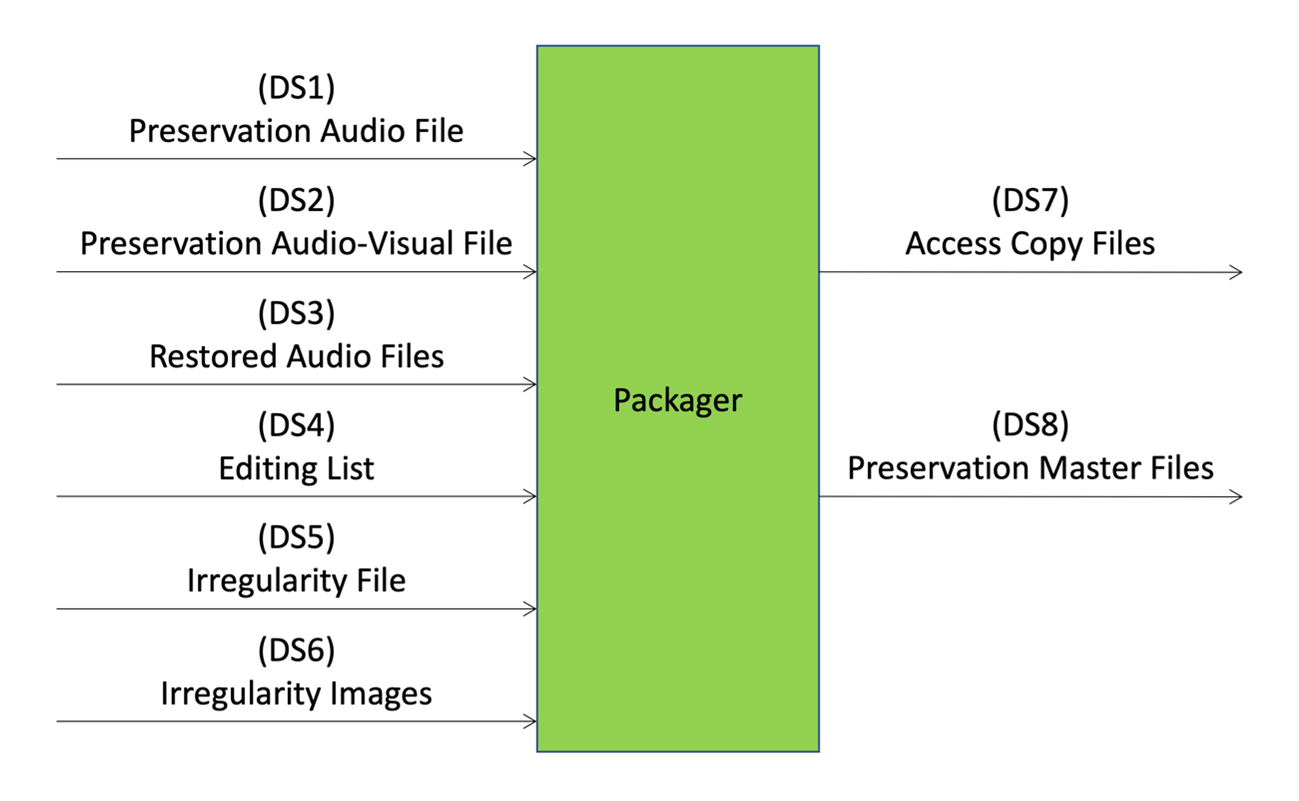
\includegraphics[width=0.9\textwidth]{img/packager.png}
    \caption{\ac{ARP} Packager}
    \label{fig:packager}
\end{figure}

Il Packager, come anticipato nella sottosezione \ref{ssec:mpai-cae-arp}, è l'ultimo \ac{AIM} ad essere eseguito e si occupa di raccogliere tutti i file elaborati e di restituire in uscita all'\ac{AIW} una cartella con la copia d'accesso dei file ed una con i file grezzi accompagnati da tutte le irregolarità trovate, vedi schema in figura \ref{fig:packager}.

Viene riportata la descrizione definita da \ac{MPAI} dei conformance tests da seguire nella tabella \ref{tab:packager-valutazione}.\footnote{Estratta dalla versione WD 0.15.2 del documento MPAI Conformance Testing per \ac{CAE}.} 
\begin{table}[H]
    \centering
    \begin{tabular}{|p{0.25\textwidth}|p{0.75\textwidth}|}
        \hline
        \textbf{Means}   &   \textbf{Actions}\\
        \hline
        \textbf{Conformance Testing Dataset}    &
            DS1: n Preservation Audio Files.\newline
            DS2: n Preservation Audio-Visual Files related to DS1.\newline
            DS3: n Restored Audio Files arrays related to DS1 coming from Tape Audio Restoration.\newline
            DS4: n Editing Lists related to DS3 coming from Tape Audio Restoration.\newline
            DS5: n Irregularity Files related to DS1 coming from Tape Irregularity Classifier.\newline
            DS6: n Irregularity Images related to DS5 coming from Tape Irregularity Classifier.\newline
            DS7: n Access Copy Files.\newline
            DS8: n Preservation Master Files.\\
        \hline
        \textbf{Procedure}  &
            1.	Feed Packager under test with DS1, DS2, DS3, DS4, DS5 and DS6.\newline
            2.	Compare the output Access Copy Files with DS7.\newline
            3.	Compare the output Preservation Master Files with DS8.\\
        \hline
        \textbf{Evaluation} &
            For a given input tuple, verify that:\newline
                1.	The output Access Copy Files contain the Restored Audio Files, the Editing List, the Irregularity File and the set of Irregularity Images in a .zip file, and is therefore equal to DS7.\newline
                2.	The output Preservation Master Files contain the Preservation Audio File, the Preservation Audio-Visual File with the audio of the Preservation Audio File, the Irregularity File and the Irregularity Images, and is therefore equal to DS8.\newline
            An error on any of the output arrays will make the Packager under test not conformant.\\
        \hline
    \end{tabular}
    \caption{Test di conformità per \ac{ARP} Packager}
    \label{tab:packager-valutazione}
\end{table}

Ci si aspetta che tutti i dataset utilizzati per eseguire i test seguano la struttura dell'albero delle cartelle come nell'esempio in figura \ref{fig:arp-filetree}.

Ad ogni esecuzione dei test è richiesto di inserire i dati nel report mostrato in tabella \ref{tab:packager-report}.
\begin{table}[H]
    \centering
    \begin{tabularx}{\textwidth}{|p{0.25\textwidth}|X|}
        
        \hline
        \textbf{Conformance Tester ID}                      &   Unique Conformance Tester Identifier assigned by MPAI\\
        \hline
        \textbf{Standard, Use Case ID and Version}          &   Standard ID and Use Case ID, Version and Profile of the standard in the form “CAE:ARP:1:0”.\\
        \hline
        \textbf{Name of AIM}                                &   Packager\\
        \hline
        \textbf{Implementer ID}                             &   Unique Implementer Identifier assigned by MPAI Store.\\
        \hline
        \textbf{AIM Implementation Version}                 &   Unique Implementation Identifier assigned by Implementer.\\
        \hline
        \textbf{Neural Network Version (optional)}          &   Unique Neural Network Identifier assigned by Implementer.\\
        \hline
        \textbf{Identifier of Conformance Testing Dataset}  &   Unique Dataset Identifier assigned by MPAI Store.\\
        \hline
        \textbf{Test ID}                                    &   Unique Test Identifier assigned by Conformance Tester.\\
        \hline
        \textbf{Actual output}                              &   Actual output provided as a matrix of n rows containing output assertions.\\
                                                            &   \begin{adjustbox}{max width=0.7\textwidth} \begin{tabular}{|c|c|c|c|c|}
            \hline
            Output                      &   Files                           &   1   &   \dots   &   n\\
            \hline
            Access Copy Files           &   Restored Audio Files            &   T/F &   \dots   &   T/F\\
                                        &   Editing List                    &   T/F &   \dots   &   T/F\\
                                        &   Irregularity File               &   T/F &   \dots   &   T/F\\
                                        &   Irregularity Images             &   T/F &   \dots   &   T/F\\
            \hline
            Preservation Master Files   &   Preservation Audio File         &   T/F &   \dots   &   T/F\\
                                        &   Preservation Audio Visual File  &   T/F &   \dots   &   T/F\\
                                        &   Irregularity File               &   T/F &   \dots   &   T/F\\
                                        &   Irregularity Images             &   T/F &   \dots   &   T/F\\
            \hline
        \end{tabular} \end{adjustbox}\\
                                                            &   Final assertion: T/F\\
        \hline
        \textbf{Execution time (optional)}                  &   Duration of test execution\\
        \hline
        \textbf{Test comment (optional)}                    &   Comments on test results and possible needed actions.\\
        \hline
        \textbf{Test Date}                                  &   yyyy/mm/dd.\\
        \hline
    \end{tabularx}
    \caption{Report da compilare ad ogni esecuzione del packager}
    \label{tab:packager-report}
\end{table}
Viene creato automaticamente il report sotto forma di file JSON contenente le informazioni conosciute dal software anche grazie all'aiuto della libreria \href{https://github.com/numirias/pytest-json-report}{pytest-json-report} che raccoglie i risultati dei test in un formato machine-readable.

Il seguente listato ne è un esempio:
\lstinputlisting[language=json, caption={Esempio di report compilato sotto forma di file JSON, \acs{AIM} Packager}]{listings/packager-report.json}


\subsection{Bugs ed altri problemi pre-esistenti} \label{ssec:packager-pre}  % moviepy vs ffmpeg (errori nel video e audio transcodifica in mp3), offset
Prima di dedicarsi alla scrittura dei test, si è verificata la corretta funzionalità del software.

Sono stati riscontrati dei problemi importanti relativi alla creazione del Preservation Audio-Visual File:

\begin{lstlisting}[language=Python, caption={Codice iniziale, creazione Preservation Audio-Visual File (Packager)}]
# Create Preservation Audio-Visual File with substituted audio
video_file = files_name + '.mov'
pvf_path = os.path.join(working_path, 'PreservationAudioVisualFile/', video_file)
try:
    audio = AudioFileClip(paf_path)
    video = VideoFileClip(pvf_path)
    # Open Irregularity File to get offset
    irregularity_file_json = open(
        os.path.join(temp_path, 'TapeIrregularityClassifier_IrregularityFileOutput2.json')
    )
    irregularity_file = json.load(irregularity_file_json)
    offset = irregularity_file['Offset']/1000
    if offset > 0:
        audio = audio.subclip(t_start=offset)
    else:
        video = video.subclip(t_start=offset)
    video = video.set_audio(audio)
    video.write_videofile(pmf_path + 'PreservationAudioVisualFile.mov', bitrate='3000k', codec='mpeg4')
    print("Preservation Audio-Visual File created")
except OSError:
    pprint(f"Preservation Audio-Visual File file '{pvf_path}' not found!", color=Color.RED)
    quit(os.EX_NOINPUT)
\end{lstlisting}

Il primo problema è relativo alla sincronizzazione del video con l'audio: l'audio deve essere anticipato se viene trovato uno scostamento A/V positivo, altrimenti deve essere anticipato il video.
Alle righe 12-16 si osserva che il comportamento non è quello richiesto: dato che a riga 16 l'offset ha valore negativo, allora \href{https://zulko.github.io/moviepy/}{MoviePy}, libreria utilizzata per eseguire editing video, farà iniziare la traccia a partire da $|offset|$ secondi prima del termine della clip.\footnote{Codice sorgente: \url{https://zulko.github.io/moviepy/_modules/moviepy/Clip.html\#Clip.subclip}}

Il secondo problema è relativo alla non specifica nel codice della codifica audio che porta la libreria MoviePy a ricadere nel comportamento di default ovvero generare un file con codifica MP3 (lossy) a \qty{44100}{\Hz} e ad avere di conseguenza, in questo caso, una transcodifica, il che non è ottimale per un software che ha come obiettivo la conservazione di documenti audio in alta qualità.

Il terzo problema invece è provocato dalla libreria \href{https://zulko.github.io/moviepy/}{MoviePy} che, per motivi sconosciuti e solo in alcuni casi, genera file corrotti nella traccia video, nello specifico che si bloccano dopo alcuni secondi.

Per risolvere questi due problemi si è scelto di sostituire MoviePy direttamente con \href{https://ffmpeg.org/}{FFmpeg}, ottenendo come risultato il seguente codice:
\begin{lstlisting}[language=Python, caption={Codice finale, creazione Preservation Audio-Visual File (Packager)}]
# Create Preservation Audio-Visual File with substituted audio
video_file = files_name + '.mov'
pvf_path = os.path.join(working_path, 'PreservationAudioVisualFile/', video_file)
try:
    # Open Irregularity File to get offset
    irregularity_file_json = open(
        os.path.join(temp_path, 'TapeIrregularityClassifier_IrregularityFileOutput2.json')
    )
    irregularity_file = json.load(irregularity_file_json)
    offset = irregularity_file['Offset']
    command_to_run = ['ffmpeg',
                      '-y', '-hide_banner', '-loglevel', 'error']
    # If offset is positive, the audio is anticipated, otherwise video is anticipated (through seek)
    if offset > 0:
        command_to_run = command_to_run + ['-i', pvf_path,
                                           '-ss', str(offset)+'ms', '-i', paf_path]
    else:
        command_to_run = command_to_run + ['-ss', str(offset * -1)+'ms', '-i', pvf_path,
                                           '-i', paf_path]
    command_to_run = command_to_run + ['-c:v', 'mpeg4', '-c:a', 'copy',
                                       '-map', '0:v', '-map', '1:a',
                                       '-b:v', '3M', '-maxrate', '4M', '-bufsize', '4M',
                                       pmf_path + 'PreservationAudioVisualFile.mov']
    subprocess.run(command_to_run)
    print("Preservation Audio-Visual File created")
except OSError:
    pprint(f"Preservation Audio-Visual File file '{pvf_path}' not found!", color=Color.RED)
    quit(os.EX_NOINPUT)
\end{lstlisting}


\subsection{Come verificare l'uguaglianza tra tracce audio} \label{ssec:packager-audio}    % fingerprinting con chromaprint, suo wrapper in python, free software e mie contribuzioni, comunicare col mantainer
Per verificare l'uguaglianza fra tracce audio, inizialmente si è provato un confronto tramite le librerie \textit{hashlib} o \textit{filecmp}, ma entrambi i test non hanno avuto successo perché in alcuni casi non è richiesto di verificare che il file sia lo stesso identico (stesso hash), ma piuttosto di controllare che il suono sia il medesimo.\footnote{La differenza si osserva, per esempio, quando si hanno 2 file, uno scostato di qualche secondo rispetto all'altro; questo è ciò che accade nel caso in esame quando si esegue la sincronizzazione audio/video.}

La soluzione trovata si basa sulla libreria \href{https://acoustid.org/chromaprint}{chromaprint}\footnote{chromaprint è la libreria che è alla base del progetto AcoustID, utilizzato nel piuttosto famoso software \href{https://musicbrainz.org/}{MusicBrainz} (\href{https://picard.musicbrainz.org/}{Picard}) che serve a taggare le proprie tracce musicali.}, la quale permette di ricavare un'impronta digitale (\textit{fingerprint}) a partire da una traccia audio in maniera da poi confrontare due impronte tra loro per ottenere una misura della somiglianza tra le rispettive tracce.    % TODO taggare va bene?

È stata utilizzata in particolare una libreria Python, la quale non è altro che un wrapper di AcoustID, chiamata \href{https://github.com/beetbox/pyacoustid}{pyacoustid} che aiuta lo sviluppatore Python esponendo direttamente le API di chromaprint ed un metodo per confrontare le impronte.

\begin{lstlisting}[language=Python, caption=Test di comparazione di due file audio tramite la loro impronta digitale]
AUDIO_THRESHOLD = 0.7   # (ratio)
# [...]
input_fingerprint = acoustid.fingerprint_file(input_paf_path)
output_fingerprint = acoustid.fingerprint_file(output_paf_path)
assert acoustid.compare_fingerprints(input_fingerprint, output_fingerprint) > AUDIO_THRESHOLD, "PreservationAudioFile.wav is not the same as input"
\end{lstlisting}

Come si può leggere dal codice, è stata scelta come soglia di somiglianza il $70\%$, non il $100\%$ perché, ad esempio, nei casi in cui è stata effettuata la sincronizzazione audio/video l'audio non è esattamente uguale; inoltre dai vari test eseguiti sui dataset forniti, questo valore ha funzionato correttamente.

Durante la scelta della soglia da adottare sono state eseguite diverse prove ed è stato verificato che, correttamente, anche nel caso dei dataset forniti, si ottengono dei risultati elevati, talvolta uguali a $1$, se i file dovrebbero essere considerati uguali, mentre in caso di file diversi si ottiene un valore tendente a $0$.\footnote{Alcune prove si possono trovare alla pagina: \url{https://github.com/albertopasqualetto/Tesi-triennale/blob/main/Notebooks/chromaprint_comparisons.ipynb}}   % non è più stata trovata una differenza in base al codec

La libreria pyacoustid, nelle prime fasi di scrittura dei test, non era ancora completamente funzionante né compresa del metodo per comparare le impronte digitali, infatti la sua versione 1.2.2, presente nella repository \href{https://pypi.org/}{PyPi}, non vedeva ancora implementata la funzione \verb|compare_fingerprints|, già presente invece nella sua repository GitHub grazie al contributo di un utente; tale implementazione era, però, non funzionante a causa di alcuni errori del codice come si può vedere dai cambiamenti applicati successivamente e descritti qui di seguito: 

\begin{lstlisting}[language=diff, caption=Correzioni applicate in pyacoustid nel codice del confronto tra impronte]
@@ -382,7 +382,7 @@ def _match_fingerprints(a: List[int], b: List[int]) -> float:       
             if biterror <= MAX_BIT_ERROR:
                 offset = i - j + bsize
                 counts[offset] += 1
-    topcount = counts.max()
+    topcount = max(counts)
     return topcount / min(asize, bsize)


@@ -399,6 +399,6 @@ def compare_fingerprints(a, b) -> float:
     # decompress fingerprints
-    a = [int(x) for x in chromaprint.decode_fingerprint(a)[0]]
-    b = [int(x) for x in chromaprint.decode_fingerprint(b)[0]]
+    a = [int(x) for x in chromaprint.decode_fingerprint(a[1])[0]]
+    b = [int(x) for x in chromaprint.decode_fingerprint(b[1])[0]]
     return _match_fingerprints(a, b)
\end{lstlisting}

Per applicare queste modifiche è stato necessario effettuare una \ac{PR}\footnote{Una \ac{PR} è una richiesta ai manutentori del codice di aggiungerne di proprio per implementare nuove funzioni o per correggere dei problemi.} sulla repository ufficiale a cui ha seguito uno scambio di messaggi con il manutentore e l'implementatore del codice;\footnote{URL della \ac{PR}: \url{https://github.com/beetbox/pyacoustid/pull/78}} questa è una pratica comune nel mondo del software libero, il quale, tra i vari vantaggi, permette di leggere il codice sorgente e contribuire con dei miglioramenti alle tecnologie che si utilizzano.\footnote{\url{https://opensource.guide/how-to-contribute/\#improve-software-you-rely-on}}
Si è contribuito a pyacoustid anche con un'altra \ac{PR} che permette l'utilizzo della libreria anche in Windows, la quale è stata implementata collaborando col manutentore.\footnote{URL della \ac{PR}: \url{https://github.com/beetbox/pyacoustid/pull/79}}

Ora la versione presente su PyPi è la 1.3.0, contenente tutte le modifiche citate.


\subsection{Come verificare l'uguaglianza tra flussi video} \label{ssec:packager-video}    % ffmpeg e psnr
Per verificare l'uguaglianza tra gli stream video è stato utilizzato il \ac{PSNR} medio tra i frame dei 2 video, calcolato tramite FFmpeg.\footnote{\url{https://ffmpeg.org/ffmpeg-all.html\#psnr}}

Il \ac{PSNR} è una misura di qualità di un'immagine compressa rispetto all'originale; viene definito come il rapporto tra la massima potenza di un segnale (immagine originale) e la potenza del rumore rispetto alla sua rappresentazione (immagine compressa).
In questo caso si utilizzano al posto delle immagini originale e compressa, i frame dei 2 video da confrontare rispettivamente.

\begin{lstlisting}[language=Python, caption=Test di comparazione di due file audio tramite il PSNR]
VIDEO_THRESHOLD = 25    # dB
# [...]
psnr_out = subprocess.run(["ffmpeg",    # video
                           "-i", input_pvf_path,
                           "-i", tmp_path / (files_name+"_PreservationAudioVisualFile_output_video.mov"),
                           "-filter_complex", "psnr",
                           "-f", "null",
                           "-"],
                          capture_output=True)
psnr_out = psnr_out.stderr.decode("utf-8")
psnr = psnr_out[psnr_out.find('average:') + 8:psnr_out.find(' ', psnr_out.find('average:'))]
print("psnr_out=", psnr)
assert psnr == 'inf' or float(psnr) > VIDEO_THRESHOLD, "PreservationAudioVisualFile.mov is not the same as input"
\end{lstlisting}

Come si può osservare dal codice, è stato individuato un \ac{PSNR} soglia di \qty{25}{\dB}, ancora una volta non è massimo (infinito) perché nei casi di sincronizzazione in cui si taglia una parte di video, si ottiene un valore minore (e nemmeno elevato) di \ac{PSNR}, ma comunque in grado di discernere video "uguali" da video veramente distinti.

Esistono altri metodi per comparare dei video e tra questi vi sono il \ac{SSIM} oppure, ancora una volta, qualche algoritmo di fingerprinting, ma si è visto che il \ac{PSNR} è funzionale allo scopo ed è il più rapido ad essere eseguito; il codice potrebbe essere migliorato per avere più certezza dell'uguaglianza, ma questo non è un problema semplice considerando che i video in questione sono identici a meno di un'eventuale taglio della parte iniziale, un'idea potrebbe essere quella di calcolare il \ac{PSNR} a ritroso e considerando i video solo per la durata del più breve, ciò però non considererebbe il caso limite di file diversi con la parte terminale in comune.


\subsection{Refactoring del codice della libreria} \label{ssec:packager-post}  % principio DRY, docstrings, unit tests, compatiblità Windows ma esecuzione docker
A termine del lavoro è stato eseguito un refactoring del codice della libreria ricalcando lo stile del \ac{TDD}.
Si è cercato di seguire il principio \ac{DRY}, ovvero di limitare la ridondanza del codice creando delle funzioni autoesplicative per ogni macro azione del codice.
Facendo ciò si è limitata la ridondanza sia all'interno dello stesso file, sia si è rimossa la duplicazione tra client e server, che ora utilizzano entrambi le funzioni di una libreria condivisa.

Per le funzioni appena citate sono stati creati degli unit tests per le funzionalità non ancora collaudate dai conformance tests.

Ove opportuno sono state scritte le docstings per le funzioni, ovvero la loro documentazione.

Sono state anche aggiunte delle strutture di controllo per assicurare l'esecuzione da capo a fine in Windows, dato che alcune funzionalità non sono supportate dal sistema operativo di Microsoft:
\begin{lstlisting}[language=diff, caption=Modifiche per permettere la compatibilità di Packager con Windows]
- quit(os.EX_CONFIG)
+ if not sys.platform.startswith(('win', 'cygwin')):
+     quit(os.EX_CONFIG)  # `os.EX_CONFIG` is not compatible with the above platforms in Python 3.10
+ else:
+     quit()
\end{lstlisting}
Ciò è stato fatto nell'ottica di garantire l'esecuzione multipiattaforma, nonostante in produzione il Packager sia eseguito in un container Linux.


\section{MPAI-CAE-ARP Audio Analyser} \label{sec:test-audioanalyser}
Successivamente è stato preso in considerazione l'\ac{AIM} Audio Analyser.

\begin{figure}[H]
    \centering
    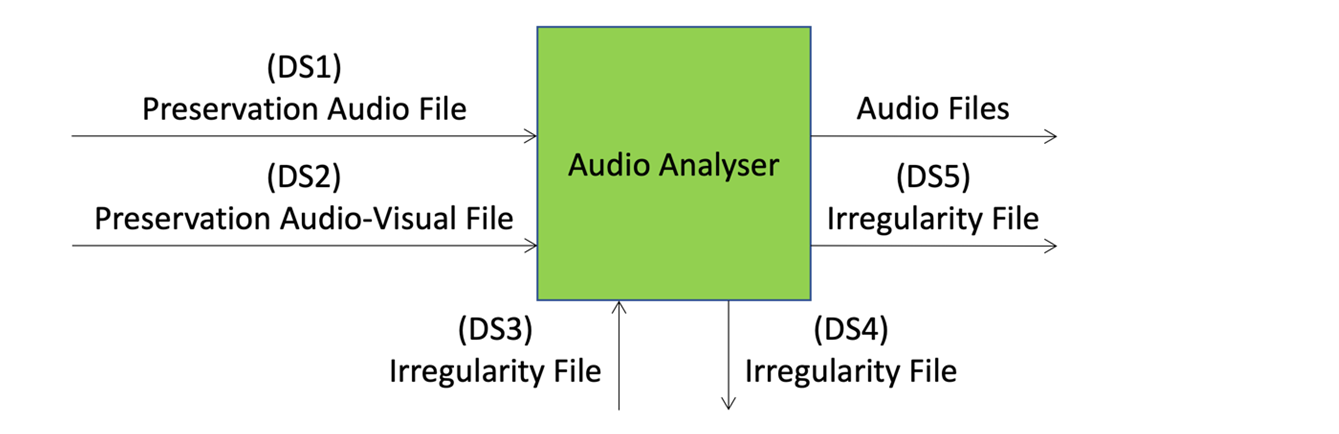
\includegraphics{img/audioanalyser.png}
    \caption{\ac{ARP} Audio Analyser}
    \label{fig:audio-analyser}
\end{figure}

L'Audio Analyser, come anticipato nella sottosezione \ref{ssec:mpai-cae-arp}, è l'\ac{AIM} che si occupa di individuare le irregolarità nell'audio, di fornirle al Video Analyser e, una volta ottenute anche le irregolarità del video, di fornirle al Tape Irregularity Classifier (il classificatore delle irregolarità), oltre a ciò si occupa di passare al classificatore appena citato anche dei frammenti di audio lunghi \qty{500}{\ms} in corrispondenza di ogni irregolarità, vedi schema in figura \ref{fig:audio-analyser}.

Viene riportata la descrizione definita da \ac{MPAI} dei conformance tests da seguire nella tabella \ref{tab:audioanalyser-valutazione}.\footnote{Estratta dalla versione WD 0.15.2 del documento MPAI Conformance Testing per \ac{CAE}.}

\begin{spacing}{1.1}
\begin{table}[H]
    \centering
    \begin{tabular}{|p{0.18\textwidth}|p{0.82\textwidth}|}
        \hline
        \textbf{Means}   &   \textbf{Actions}\\
        \hline
        \textbf{Conformance Testing Dataset}    &
            DS1: n* Preservation Audio Files.\newline
            DS2: n Preservation Audio-Visual Files related to DS1.\newline
            DS3: n Irregularity Files related to DS2.\newline
            DS4: n output Irregularity Files in the format of port IrregularityFileOutput\_1 with all Irregularities correctly identified.\newline
            DS5: n output Irregularity Files in the format of port IrregularityFileOutput\_2 with the real offset and all Irregularities correctly identified and included from DS3.\newline
            \newline
            \footnotesize* A reasonable n for testing is 5<n<=10, since each file generates multiple irregularities to classify\\
        \hline
        \textbf{Procedure}  &
            1.	Feed Audio Analyser under test with DS1, DS2 and DS3.\newline
            2.	Compare the computed offsets with the ones contained in DS5.\newline
            3.	Analyse the Irregularity Files resulting from port IrregularityFileOutput\_1.\newline
            4.	Analyse the Irregularity Files resulting from port IrregularityFileOutput\_2.\\
        \hline
        \textbf{Evaluation} &
            	1.	Verify the conditions:\newline
            	   a.	The Irregularity Files are syntactically correct and conforming to the JSON schema provided in CAE Technical Specification.\newline
            	   b.	All Irregularities from DS3 are included in the Irregularity Files coming from port IrregularityFileOutput\_2.\newline
            	   c.	$|O_c - O_r| < 3 \times \lceil\frac{1000}{FPS_{DS3}}\rceil ms$, where $O_c$ is the offset computed by the Audio Analyser under test, $O_r$ is the real offset and $FPS_{DS3}$ is the number of frames per second at which the DS3 video has been recorded.\newline
            	   d.	All output Audio Files are conforming to RF64 file format.\newline
            	   e.	For each of the n tuples of input records, the output Audio Files are extracted from the corresponding input Preservation Audio File at the Time Labels indicated in the Irregularity File coming from port IrregularityFileOutput\_2.\newline
            	2.	By inspecting the Irregularity Files resulting from port IrregularityFileOutput\_1, for each of the n tuples of input records, compute the values of Recall (R) and Precision (P).\newline
            	3.	Compute the average value of Recall ($\Tilde{R}$) and Precision ($\Tilde{P}$) measures obtained at point 2.\newline
            	4.	Accept the AIM under test if:\newline
                	a.	$\Tilde{R} > 0.9$\newline
                	b.	$\Tilde{P} > 0.9$\\
        \hline
    \end{tabular}
    \caption{Test di conformità per \ac{ARP} Audio Analyser}
    \label{tab:audioanalyser-valutazione}
\end{table}

Ci si aspetta che tutti i dataset utilizzati per eseguire i test seguano la struttura dell'albero delle cartelle come nell'esempio in figura \ref{fig:arp-filetree}.

Ad ogni esecuzione dei test è richiesto di inserire i dati nel report mostrato in tabella \ref{tab:audioanalyser-report}.
\begin{table}[H]
    \centering
        \begin{tabularx}{\textwidth}{|p{0.3\textwidth}|X|}
            \hline
            \textbf{Conformance Tester ID}                      &   Unique Conformance Tester Identifier assigned by MPAI\\
            \hline
            \textbf{Standard, Use Case ID and Version}          &   Standard ID and Use Case ID, Version and Profile of the standard in the form “CAE:ARP:1:0”.\\
            \hline
            \textbf{Name of AIM}                                &   Audio Analyser\\
            \hline
            \textbf{Implementer ID}                             &   Unique Implementer Identifier assigned by MPAI Store.\\
            \hline
            \textbf{AIM Implementation Version}                 &   Unique Implementation Identifier assigned by Implementer.\\
            \hline
            \textbf{Neural Network Version (optional)}          &   Unique Neural Network Identifier assigned by Implementer.\\
            \hline
            \textbf{Identifier of Conformance Testing Dataset}  &   Unique Dataset Identifier assigned by MPAI Store.\\
            \hline
            \textbf{Test ID}                                    &   Unique Test Identifier assigned by Conformance Tester.\\
            \hline
            \textbf{Actual output}                              &   Actual output provided as a matrix of n rows containing R and P values.\\
                                                                &   \begin{adjustbox}{max width=0.65\textwidth} \begin{tabular}{|c|c|c|}
                \hline
                Tuple \# &   R   &   P\\
                \hline
                1       &   Measure 1   &   Measure 1\\
                \hline
                \dots   &   \dots       &   \dots\\
                \hline
                n       &   Measure n   &   Measure n\\
                \hline
            \end{tabular} \end{adjustbox} \smallskip\\
            \hline
            \textbf{Execution time (optional)}                  &   Duration of test execution.\\
            \hline
            \textbf{Test comment (optional)}                    &   -\\
            \hline
            \textbf{Test Date}                                  &   yyyy/mm/dd.\\
            \hline
        \end{tabularx}
    \caption{Report da compilare ad ogni esecuzione dell'Audio Analyser.}
    \label{tab:audioanalyser-report}
\end{table}
\end{spacing}
Il report viene compilato automaticamente in un file JSON come spiegato anche per il Packager (sottosezione \ref{ssec:packager-pre}).
Un esempio è riportato di seguito:
\lstinputlisting[language=json, caption={Esempio di report compilato sotto forma di file JSON, \acs{AIM} Audio Analyser}]{listings/audioanalyser-report.json}


\subsection{Problemi pre-esistenti} \label{ssec:audioanalyser-pre}  % typos, video analyser usa : invece di . e workaround, in Windows scipy.signal.correlate da overflow perche tipo di default per numpy è int32, test non funzionanti
Alla prima esecuzione del modulo, ancora prima di scrivere i test richiesti, si è notato che l'offset calcolato fosse estremamente diverso da quello fornito nei dataset di esempio, nello specifico si osservava addirittura uno scostamento di segno opposto. Indagando si è riscontrato che il problema si presentasse solo nel caso di utilizzo del codice su piattaforme Windows ed infine si è visto che l'errore fosse dato dal fatto che il tipo di dato di default per NumPy in Windows è \texttt{int32} anche in macchine a 64 bit, mentre in ambiente Unix (ancora una volta si far riferimento a problemi non riscontrabili in produzione) il default è \texttt{int64}; passando il tipo necessario manualmente, il problema di overflow alla chiamata di \texttt{scipy.signal.correlate} non si presenta più.\footnote{\url{https://github.com/numpy/numpy/issues/9464}}
Questa problematica risiede nella libreria \texttt{mpai-cae-arp}, la quale viene discussa nella sezione \ref{sec:lib-mpaicaearp}.   % TODO dovrei nominare prima scipy.signal.correlate?

Sono stati sistemati degli errori di battitura, alcuni dei quali impedivano il funzionamento del codice (vedi l'uso ambiguo di Pydantic precedentemente permesso alla sottosezione \ref{ssec:mpaicaearp-pydantic})

È stata aggiornata la versione richiesta della libreria mpai-cae-arp su cui sono basati tutti gli \ac{AIM} di \ac{ARP}:
\begin{lstlisting}[language=diff, caption={Aggiornamento della libreria \texttt{mpai-cae-arp} in Audio Analyser, file \texttt{pyproject.toml}}]
@@ -21,5 +21,5 @@ 
    pandas = "^2.0.0"
    scikit-learn = "^1.2.2"
    grpcio-tools = "^1.53.0"
-   mpai-cae-arp = "^0.3.0"
+   mpai-cae-arp = "^0.5.0"
    ffmpeg-python = "^0.2.0"
\end{lstlisting}
Si nota che la specifica \verb|^0.3.0| (basata sul \href{https://semver.org/lang/it/}{versionamento semantico}) permette solo le versioni $\ge0.3.0, <0.4.0$, quindi l'aggiornamento fino a prima della successiva MINOR, differendo dal normale funzionamento in presenza di versioni con MAJOR$\ge1$ ($\ge1.0.0$) per cui si permette l'aggiornamento fino a prima della successiva MAJOR.\footnote{Fonte: \href{https://python-poetry.org/docs/dependency-specification/\#caret-requirements}{documentazione di Poetry}.}

Infine nel codice dei test si dovrà fronteggiare il fatto che, in maniera incorretta, nel video analyser si utilizzano come divisore tra secondi e millisecondi i due punti (:) (si può vedere nei file \verb|*_IrregularityFileOutputN.json|), quindi, alla lettura di file contenenti irregolarità provenienti dal video analyser, si dovranno applicare delle soluzioni per aggirare il problema ed inoltre si vedranno fallire i test che chiedono di verificare la sintassi dello schema JSON nel caso contengano le irregolarità già citate.


\subsection{Come verificare che l'offset calcolato sia compatibile con quello reale} \label{ssec:audioanalyser-offset}   % formula fornita + ffprobe
Nella tabella di valutazione \ref{tab:audioanalyser-valutazione} al punto 1.c viene richiesto di controllare che lo scostamento calcolato dall'Audio Analyser sia sufficientemente vicino quello reale, fornito nel dataset 5.
Per fare ciò si richiede che la differenza in valore assoluto tra i 2 offset sia minore del tempo necessario a mostrare 3 frame del Preservation Audio-Visual File in millisecondi e si calcola tramite la seguente disuguaglianza:
\begin{equation}
    |O_c - O_r| < 3 \times \big\lceil\frac{1000}{FPS_{DS3}}\big\rceil ms
\end{equation}
dove $O_c$ è l'offset calcolato, $O_r$ è l'offset reale e $FPS_{DS3}$ sono gli FPS del Preservation Audio-Visual File.

Gli FPS del video sono ottenuti tramite \href{https://ffmpeg.org/ffprobe.html}{ffprobe}, una utility di FFmpeg votata all'acquisizione di informazioni da file multimediali, tramite la richiesta di mostrare lo stream \verb|r_frame_rate|.\footnote{Si usa il comando \texttt{ffprobe -v 0 -of csv=p=0 -select\_streams v -show\_entries stream=r\_frame\_rate video\_path.mov}}

Il codice utilizzato è il seguente:
\begin{lstlisting}[language=Python, caption={Codice del test di conformità sulla differenza tra scostamento reale e calcolato, Audio Analyser}]
@pytest.mark.parametrize("files_name", files_names)
def test_offset_difference(files_name: str):
    """Conformance testing specification point c.

    Test if the offset difference between Audio Analyser and DS5 real offset is small.
    """
    aa_if1_path = temp_path / files_name / "AudioAnalyser_IrregularityFileOutput1.json"
    test_if2_path = oldify(temp_path / files_name / "AudioAnalyser_IrregularityFileOutput1.json")
    assert aa_if1_path.is_file(), "AudioAnalyser_IrregularityFileOutput1.json not found"
    with open(aa_if1_path, "r") as aa_if_file:
        aa_if_dict = json.load(aa_if_file)
    with open(test_if2_path, "r") as test_if_file:
        test_if_dict = json.load(test_if_file)
    aa_offset = int(aa_if_dict["Offset"])
    real_offset = int(test_if_dict["Offset"])

    out = subprocess.run(["ffprobe", "-v", "0", "-of", "csv=p=0", "-select_streams", "v", "-show_entries", "stream=r_frame_rate", str(working_path / "PreservationAudioVisualFile" / (files_name+".mov"))], capture_output=True)
    rate = out.stdout.decode("utf-8").split('/')
    fps = int(rate[0]) / int(rate[1])
    
    assert abs(aa_offset - real_offset) < 3 * math.ceil(1000 / fps), f"Offset difference is too big: {abs(aa_offset - real_offset)}ms"
\end{lstlisting}


\subsection{Come verificare che dei file siano in formato WAV} \label{ssec:audioanalyser-wav}    % RF64 ma in realtà va bene wav; libreria filetype, magic numbers, MIME
Nella tabella \ref{tab:audioanalyser-valutazione} al punto 1.d viene richiesto di controllare che i segmenti audio estratti dall'Audio Analyser siano in formato RF64: un formato compatibile col WAV; in realtà in questo caso è sufficiente verificare che tali segmenti siano in formato WAV.

Per fare ciò è stata utilizzata la libreria Python \href{https://github.com/h2non/filetype.py}{filetype} che legge i magic numbers: delle stringhe costanti nell'header di un file utilizzati per identificarne la tipologia.
La firma di un WAV in formato esadecimale è "\texttt{52 49 46 46 ?? ?? ?? ?? 57 41 56 45}".\footnote{Gli \texttt{??} indicano che i valori in quelle posizioni non sono fissi.}
La libreria citata cerca di indovinare il tipo del file e ne restituisce il tipo \acs{MIME}, \texttt{audio/x-wav} nel caso del WAV.\footnote{\acfi{MIME} è uno standard che estende le email e fornisce il supporto a dati diversi dal solo testo. Il suo \texttt{Content-Type} indica il tipo di dato.}


\subsection{Come verificare che la classificazione sia coerente} \label{ssec:audio-analyser-classificazione}    % non necessario ma utile per capire che l'IA non da sempre stessi risultati, output utilizzati per gli altri test, recall, precision
Per verificare se la rilevazione e la classificazione delle irregolarità sono coerenti con il dataset di test, è stata creata la funzione \verb|check_classification_results| che confronta 2 dizionari contenenti irregolarità e restituisce il numero di elementi diversi e dove si trovano queste diversità:
\begin{lstlisting}[language=Python, caption=Codice che testa la costanza dei risultati della classificazione in Audio Analyser]
def check_classification_results(if_dict_1: dict, if_dict_2: dict, print_differences: bool = False) -> (bool, int, int, int):
    """
    Check if the irregularity files' classification results in `if_dict_1` are exactly equal to `if_dict_2`.

    Parameters
    ----------
    if_dict_1 : dict
        First irregularity file dictionary (first file to compare).
    if_dict_2 : dict
        Second irregularity file dictionary (second file to compare).
    print_differences : bool, optional
        If True, print the differences between the two files, by default False.

    Returns
    -------
    tuple[bool, int, int, int]
        Tuple of:
            1) if the two files are exactly equal;
            2) number of elements in common;
            3) number of extra elements in the first file;
            4) number of extra elements in the second file.
    """
    def check_all_combinations(list1: list[dict], idxs1: list[int], list2: list[dict], idxs2: list[int]) -> (int | None, int | None):
        """
        Check if any combination of 2 elements with specified indexes in two different lists is equal and return the indexes of the first equal elements found.
        # [...]
        """
        def filtered_dict(dict_obj: dict, filter: list) -> dict:
            # [...]

        # [...]

    exact_equality = True
    found_n = 0
    extra_in_1 = 0
    extra_in_2 = 0
    irrs_1 = if_dict_1["Irregularities"]
    irrs_1.sort(key=lambda irr: int(irr["TimeLabel"].replace(":", "").replace(".", "")))  # FIXME workaround for ":" timelabel problem from video analyser
    irrs_2 = if_dict_2["Irregularities"]
    irrs_2.sort(key=lambda irr: int(irr["TimeLabel"].replace(":", "").replace(".", "")))

    timelabels_1 = [irr["TimeLabel"] for irr in irrs_2]
    for timelabel in list(dict.fromkeys(timelabels_1)):     # remove duplicates
        irrs_1_idxs = get_irr_idxs_by_timelabel(irrs_1, timelabel)
        irrs_2_idxs = get_irr_idxs_by_timelabel(irrs_2, timelabel)

        while True:
            irr_1_idx, irr_2_idx = check_all_combinations(irrs_1, irrs_1_idxs, irrs_2, irrs_2_idxs)
            if irr_1_idx or irr_2_idx:  # first check exact equality
                pass
            else:  # then the others remained as couples (equal length already checked)
                if not len(irrs_1_idxs) or not len(irrs_2_idxs):
                    break
                exact_equality = False
                irr_1_idx = irrs_1_idxs[0]
                irr_2_idx = irrs_2_idxs[0]
                if print_differences:
                    print("Irregularity", irrs_1[irr_1_idx], "\n\tnot exactly equal to\n\t", irrs_2[irr_2_idx])
            found_n += 1
            del irrs_1[irr_1_idx]
            del irrs_2[irr_2_idx]
            irrs_1_idxs.remove(irr_1_idx)
            irrs_2_idxs.remove(irr_2_idx)
            irrs_1_idxs = [idx - 1 if idx > irr_1_idx else idx for idx in irrs_1_idxs]
            irrs_2_idxs = [idx - 1 if idx > irr_2_idx else idx for idx in irrs_2_idxs]
        if len(irrs_2_idxs):
            extra_in_2 += len(irrs_2_idxs)

    extra_in_1 += len(irrs_1)

    return exact_equality, found_n, extra_in_1, extra_in_2
\end{lstlisting}

Quando si ha a che fare con algoritmi basati sul machine learning è la norma avere risultati non deterministici per via della componente di casualità che spesso vi è inserita.
Infatti il test che verifica l'esatta uguaglianza tra le 2 collezioni di irregolarità (\verb|test_audio_classification|) lo si è sempre visto fallire durante le sue esecuzioni, infatti esso non è richiesto dal documento descrivente i test di conformità.
Ciò che è richiesto e che si basa sul codice appena citato, invece, è di controllare che tutte e sole le irregolarità presenti nel file di test siano presenti anche nel file in output ad una nuova esecuzione dell'Audio Analyser e che siano correttamente estratti i frammenti di audio agli istanti di tempo richiesti (punto 1.e di \ref{tab:audioanalyser-valutazione}) e che inoltre la precisione ed il recupero\footnote{Precisione e recupero (\textit{Precision} e \textit{Recall}) sono entrambe metriche sulle prestazioni di una classificazione: $Precision=\frac{True\ Positives}{True\ Positives + False\ Positives}$; $Recall=\frac{True\ Positives}{True\ Positives + False\ Negatives}$.} medi delle irregolarità trovate rispetto al dizionario delle irregolarità di riferimento, il dataset 4, siano entrambi $>0.9$ considerando l'istante di tempo ed i canali audio a cui appartengono le irregolarità (punto 2 di \ref{tab:audioanalyser-valutazione}).


\section{Parallelizzare o no? confronto di velocità} \label{sec:parallelizzazione}
Il plugin di pytest \href{https://pytest-xdist.readthedocs.io/}{pytest-xdist}, già citato nella sottosezione \ref{ssec:pytest}, permette di parallelizzare l'esecuzione dei test.

I test di conformità sono stati eseguiti più volte su una macchina Windows 11 con una CPU Intel i7-1165G7 e 16 GB di RAM DDR4 a 3200 MHz, sia in modalità sequenziale, sia abilitando la parallelizzazione mediante l'opzione \texttt{-n auto} (numero di workers uguale al numero di CPUs disponibili) inserita nei files \texttt{pytest.ini} e si è osservato innanzitutto che gran parte del tempo utilizzato consiste nell'esecuzione dell'\ac{AIM} (grafici \ref{fig:grafico-distribuzione-tempo-packager} e \ref{fig:grafico-distribuzione-tempo-audioanalyser}), i quali non sono affetti dall'abilitazione della parallelizzazione ed inoltre che non c'è un vantaggio tangibile ad abilitarla perché la differenza di durata tra le due modalità è spesso quasi nulla.
Nel caso del Packager, come si osserva nel grafico in figura \ref{fig:grafico-parallelo-vs-sequenziale-packager}, i tempi di esecuzione sono comparabili, sebbene si noti una tendenza ad ottenere tempi leggermente minori con l'esecuzione in parallelo, come si può notare anche nel grafico \ref{fig:grafico-distribuzione-tempo-packager}. Per quanto concerne l'Audio Analyser, invece, si osserva nel grafico \ref{fig:grafico-distribuzione-tempo-audioanalyser} che più del 99\% della durata totale è occupata dall'esecuzione dell'\ac{AIM} stesso e che il tempo di esecuzione dei test è nell'ordine del secondo; in questo periodo così ridotto il tempo richiesto per generare e gestire i worker è decisamente rilevante, infatti si osserva che il tempo di esecuzione più che raddoppia in media abilitando la parallelizzazione. 
Una rappresentazione dei dati è presente in figura \ref{fig:test-grafici-tempo}.\footnote{Dati grezzi: \url{https://github.com/albertopasqualetto/Tesi-triennale/blob/main/Notebooks/res/pkg_timings.json}, \url{https://github.com/albertopasqualetto/Tesi-triennale/blob/main/Notebooks/res/aa_timings.json};\\
grafici e calcoli eseguiti nel notebook Python: \url{https://github.com/albertopasqualetto/Tesi-triennale/blob/main/Notebooks/create_graphs.ipynb}}

\begin{figure}[h]
     \centering
     \begin{subfigure}{0.49\textwidth}
         \centering
         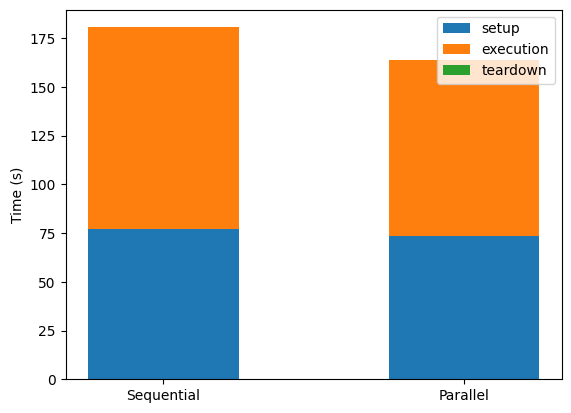
\includegraphics[width=\textwidth]{img/packager-stacked-bar-graph.png}
         \caption{Distribuzione dei tempi tra setup (esecuzione \ac{AIM}), tests e teardown (pulizia files); \ac{AIM} Packager}
         \label{fig:grafico-distribuzione-tempo-packager}
     \end{subfigure}
     \hfill
     \begin{subfigure}{0.49\textwidth}
         \centering
         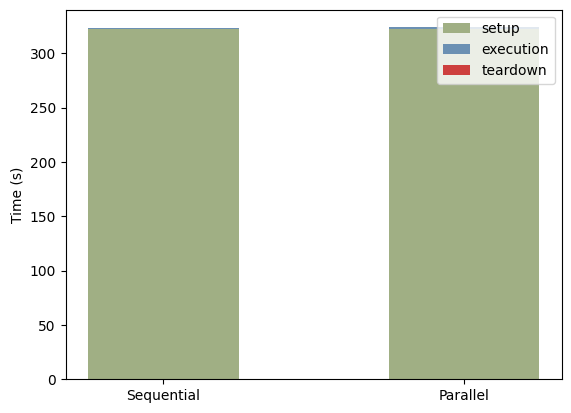
\includegraphics[width=\textwidth]{img/audioanalyser-stacked-bar-graph.png}
         \caption{Divisione dei tempi tra setup (esecuzione \ac{AIM}), tests e teardown (pulizia files); \ac{AIM} Audio Analyser}
         \label{fig:grafico-distribuzione-tempo-audioanalyser}
     \end{subfigure}
     \par\bigskip
     \begin{subfigure}{0.49\textwidth}
         \centering
         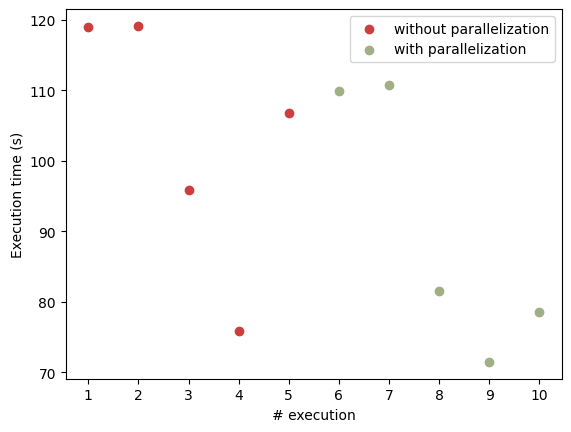
\includegraphics[width=\textwidth]{img/packager-scatter-parallelization.png}
         \caption{Tempo di esecuzione, parallelo vs sequenziale; \ac{AIM} Packager}
         \label{fig:grafico-parallelo-vs-sequenziale-packager}
     \end{subfigure}
     \hfill
     \begin{subfigure}{0.49\textwidth}
         \centering
         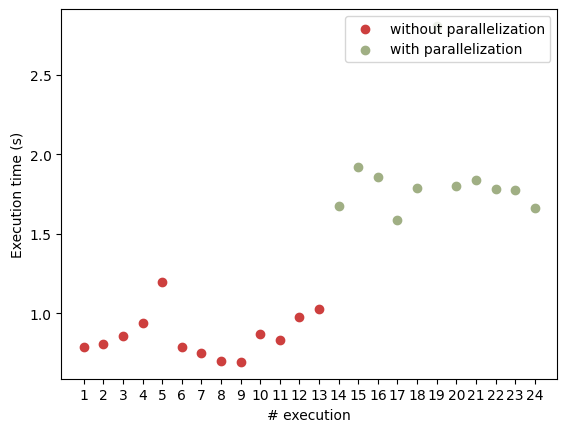
\includegraphics[width=\textwidth]{img/audioanalyser-scatter-parallelization.png}
         \caption{Tempo di esecuzione, parallelo vs sequenziale; \ac{AIM} Audio Analyser}
         \label{fig:grafico-parallelo-vs-sequenziale-audioanalyser}
     \end{subfigure}
        \caption{Tempi di esecuzione dei test eseguiti sui dataset relativi a 2 nastri}
        \label{fig:test-grafici-tempo}
\end{figure}

Si è scelto di disabilitare la parallelizzazione a causa degli scarsi risultati ottenuti con essa abilitata e per consentire l'utilizzo dei CPU cores, ora liberi, agli altri programmi.
Ciò non toglie che con un numero maggiore di pacchetti di dataset, la parallelizzazione potrebbe diventare più rilevante in termini di tempo e che si potrebbe considerare di supportarla anche nella fase di esecuzione dell'\ac{AIM} che, come visto, è molto rilevante nel computo totale di tempo utilizzato.


\section{Libreria \texttt{mpai-cae-arp}} \label{sec:lib-mpaicaearp} % a cosa serve
La libreria \href{https://pypi.org/project/mpai-cae-arp/}{mpai-cae-arp} contiene le classi, le costanti e le funzioni su cui si basano tutti gli \acp{AIM} di \ac{ARP} e che permettono loro di interoperare.
Per via della sua ampia influenza, alcuni problemi relativi a questa libreria sono stati discussi in altre sezioni (vedi \ref{ssec:audioanalyser-pre}).


\subsection{I problemi di Pydantic} \label{ssec:mpaicaearp-pydantic}    % che ha portato a dover aggiornare i moduli
È stato risolto un problema relativo all'uso non univoco di \href{https://docs.pydantic.dev/1.10/}{Pydantic}, il suo scopo principale all'interno di \ac{ARP} è quello di fornire alias corrispondenti alla nomenclatura richiesta dalle specifiche tecniche per i parametri delle funzioni in maniera tale da utilizzare il nome dell'alias per l'output verso file (\texttt{EditingList.json}, \verb|*_IrregularityFileOutputN.json|, \dots); in precedenza l'utilizzo del nome del parametro o del suo alias non era regolato e questo ha portato a degli errori che impedivano la corretta esecuzione del software.
La risoluzione applicata consiste nell'utilizzo di \verb|serialization_alias| al posto di \texttt{alias}, dato l'utilizzo primario degli alias.

Contestualmente, per favorire l'utilizzabilità nel futuro dell'applicativo, oltre che per limitarne la presenza di bug, si è scelto di aggiornare la libreria alla successiva major release (\verb|^2.3.0|).

Queste modifiche implicano il dover migrare \ac{ARP}, modificando i nomi dei campi utilizzati in tutti gli \acp{AIM} ed impedendo la retrocompatibilità.


\subsection{Bugfix: formato incorretto delle EditingList scritte su file} \label{ssec:mpaicaearp-formato-editinglist}
Un bug presente nel codice di questa libreria salvava nel filesystem dei file con una formattazione errata, un esempio ne è l'\texttt{EditingList.json} che veniva salvato nella seguente maniera:
\lstinputlisting[language=json, caption=\texttt{EditingList.json} salvato tramite la precedente modalità (errata): contiene solo una stringa]{listings/EditingList-badformat.json}
Il JSON di cui sopra è composto da una sola stringa che contiene la rappresentazione dell'oggetto Python ed i caratteri di escape mostrati, ciò portava al fallimento del relativo test di conformità del Packager (\ref{sec:test-packager}).

Il problema risiedeva nella chiamata di \texttt{json.dump} sulla stringa contenente l'oggetto da salvare in JSON generata da \texttt{model.json} (in Pydantic V2 chiamata \verb|model.model_dump_json|), questo comportamento probabilmente non era chiaro all'autore di questo codice per via del suo nome fuorviante; utilizzando, invece, la funzione di Pydantic V2 \verb|model.model_dump|, chiamata con parametro \texttt{mode='json'} per abilitare la serializzazione degli oggetti presenti nei campi della classe, si ottiene un dizionario Python che può essere scritto correttamente su file JSON (in Pydantic V1 la funzione corrispondente sarebbe stata \texttt{model.dict}, ma essa non fornisce la possibilità di serializzare gli oggetti).
Ora il file precedente appare correttamente come:
\lstinputlisting[language=json, caption=\texttt{EditingList.json} salvato tramite l'attuale modalità (corretta): contiene il dizionario con i suoi valori serializzati]{listings/EditingList-goodformat.json}


\subsection{Bugfix: oggetti \texttt{AudioWave} non funzionanti, overflow e problemi con tracce a singolo canale} \label{ssec:mpaicaearp-audiowave}  % e fare riferimento a dtype del suo buffer nominato sopra
La problematica di overflow limitata ai sistemi Windows descritta alla sottosezione \ref{ssec:audioanalyser-pre} è stata corretta col seguente codice:
\begin{lstlisting}[language=diff, caption=Risoluzione del problema di overflow degli oggetti AudioWave]
@@ -202,7 +202,7 @@ class AudioWave:
  data = np.array([
      int.from_bytes(raw_data[i:i + bit // 8], byteorder='little', signed=True)
      for i in range(0, len(raw_data), bit // 8)
- ])
+ ], dtype=np.int64)  # int32 (default in Windows) leds to overflow
  data = np.reshape(data, (-1, channels))
  return AudioWave(data, bit, channels, samplerate)
\end{lstlisting}

Questo, però, non era l'unico problema della classe AudioWave, infatti non erano supportate le tracce a singolo canale dato che l'indicizzazione di NumPy (operatore \texttt{[ ]}) non permette di operare su un array 1D come se fossero multidimensionali (ad esempio indicando il primo canale con \texttt{array[:,1]}).
\begin{lstlisting}[language=diff, caption=Modifiche ad AudioWave.get\_channel che permettono di utilizzarlo con tracce ad 1 canale]
@@ -369,39 + 369, 43 @@ class AudioWave:
  def get_channel(self, channel: int):
      # [...]
      if channel not in range(self.channels):
          raise IndexError("Channel not found")
-     return AudioWave(self.array[:, channel], self.bit, 1, self.samplerate)
+  
+     if self.channels == 1:
+         return AudioWave(self.array.squeeze(), self.bit, 1, self.samplerate)
+     else:
+         return AudioWave(self.array[:, channel], self.bit, 1, self.samplerate)
\end{lstlisting}
È necessario, perciò, introdurre una condizione sul numero di canali presenti e, nel caso ve ne sia uno solo, non operare con l'indicizzazione, come si può osservare dal codice mostrato.


\subsection{Aggiornamenti di versione} \label{ssec:mpaicaearp-aggiornamenti}
Per lo stesso motivo descritto nella sottosezione \ref{ssec:mpaicaearp-pydantic}, non solo Pydantic è stato aggiornato, ma anche le altre librerie necessarie.

La libreria \href{https://librosa.org/}{librosa} (analisi audio) richiede la libreria \href{https://numba.pydata.org/}{Numba} (compilatore JIT) che, a sua volta, richiede \href{https://llvmlite.readthedocs.io/en/latest/}{llvmlite} (Python bindings per LLVM: un'infrastruttura di compilazione) e \href{https://numpy.org/}{NumPy} (supporto ed alta efficenza computazionale per array e matrici di grandi dimensioni e funzioni matematiche); tutte queste librerie sono state aggiornate all'ultima versione compatibile tra loro, rimuovendo la dipendenza diretta \verb|llvmlite = "^0.39.1"| ed il blocco alla versione di NumPy 1.23.3 precedentemente impostati.
\begin{lstlisting}[language=diff, caption={\texttt{pyproject.toml}, aggiornamento delle dipendenze}]
@@ -9,8 +9,7 @@
  [tool.poetry.dependencies]
  python = "^3.10"
- numpy = "1.23.3"
+ numpy = "~1.24.4"   # because of numba (from librosa) requirement <=1.24
- pydantic = "^1.10.7"
+ pydantic = "^2.3.0"
  pyyaml = "^6.0"
- llvmlite = "^0.39.1" 
- librosa = "^0.10.0.post2"
+ librosa = "^0.10.1"
  grpcio-tools = "^1.53.0"
\end{lstlisting}
Questa modifica è possibile solo in seguito all'1 maggio 2023 (data successiva all'ultimo commit presente nella repository prima dell'inizio di questo lavoro), quando le librerie citate hanno introdotto la cross-compatibilità tra le nuove versioni.\footnote{Dipendenza di librosa da Numba: \url{https://github.com/librosa/librosa/blob/43d4427f7a389acc79b5be3c924646701f19bb46/setup.cfg\#L67};\\
Dipendenze di Numba da llvmlite e NumPy: \url{https://github.com/numba/numba/blob/596e8a55334cc46854e3192766e643767bd7c934/setup.py\#L367};\\
Numba 0.57 introduce il supporto a Python 3.11 e NumPy 1.24: \url{https://numba.readthedocs.io/en/stable/release-notes.html\#version-0-57-0-1-may-2023};\\
llvmlite 0.40.0 introduce il supporto a Python 3.11: \url{https://llvmlite.readthedocs.io/en/latest/release-notes.html\#v0-40-0-may-1-2023}.}

Questi aggiornamenti hanno permesso la possibilità, prima non presente, di utilizzare la libreria, e quindi di conseguenza \ac{ARP} con la versione di Python 3.11, rendendo la libreria più "a prova di futuro".
